\section{Introduction}
\ToDo{Incomplete section!}

The system is built as a service-oriented architecture \cite{neuman2015building}.
The functionality is decomposed into a set of independent, self-contained microservice modules which communicate with each other via an API.

By splitting the monolithic application into smaller modules and decoupling interdependencies (between apps, dev teams, technologies, environments, and tooling), the system gains in terms of scalability, parallel development, easier debugging, and complexity isolation.

\begin{figure}[!ht]
\centering
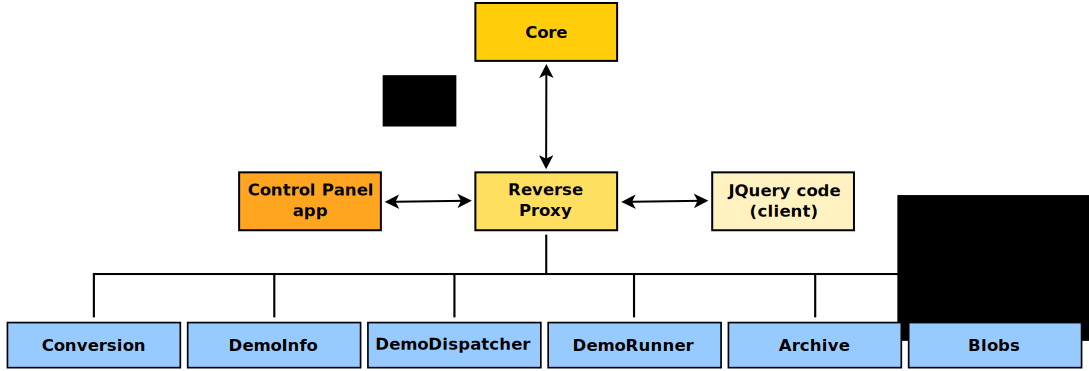
\includegraphics[width=0.8\linewidth]{architecture/images/architecture.pdf}
\caption{Modular system architecture.} 
\label{fig:architecture}
\end{figure}
